\usetikzlibrary{arrows.meta,
                chains,
                positioning,
                quotes,
                shapes.geometric}

\tikzset{FlowChart/.style={% this style can be used also at other flowcharts, 
                           % just call it with "FlowChart", see picture code below
startstop/.style = {rectangle, rounded corners, draw, fill=red!30,
                    minimum width=3cm, minimum height=1cm, align=center,
                    on chain, join=by arrow},
  process/.style = {rectangle, draw, fill=orange!30,
                    text width=5cm, minimum height=1cm, align=center,
                    on chain, join=by arrow},
 decision/.style = {diamond, aspect=1.5, draw, fill=green!30,
                    minimum width=3cm, minimum height=1cm, align=center,
                    on chain, join=by arrow},
       io/.style = {trapezium, trapezium stretches body,   % not used in your flowchart
                    trapezium left angle=70, trapezium right angle=110,
                    draw, fill=blue!30,
                    minimum width=3cm, minimum height=1cm,
                    text width =\pgfkeysvalueof{/pgf/minimum width}-2*\pgfkeysvalueof{/pgf/inner xsep},
                    align=center,
                    on chain, join=by arrow},
    arrow/.style = {thick,-Triangle}
                        }
        }% end of tikzset
% --------------------------------------------------------------
\begin{chapter}{Global Sensitivity Analysis for Stochastic Computer Models}
\section{Introduction}
Computer modelling is a standard technique in complex engineering problems. However, even if a model is built upon well tested assumptions there is still the question of what values certain parameters should take. Often, this will be obvious. It is well understood that close to the earth's surface that the gravity of earth takes the value $g = 9.81ms^{-2}$. However for complex engineering projects implementing new technologies, the values that parameters should take are not known --- they are uncertain. This input uncertainty means that, even for deterministic computer simulations, the output is also uncertain. This leads to the questions such as \textit{``How much does that uncertainty really matter?''} or \textit{``Which inputs are contributing the most to output uncertainty?''}. This is best answered by considering how the uncertainty in parameters (inputs) affects the uncertainty in key model outputs.

A fairly basic approach to considering the impact of input uncertainty is a scenario analysis  \citep{Zhang2012, Grewal2013} however this does not consider how likely each of the scenarios are; it could be very easy to plan for catastrophic events even when they are practically impossible. Another approach is one-at-a-time (OAT) sensitivity analysis in which each uncertain parameter is varied whilst keeping all other parameters fixed at a nominal value \citep{Holvoet2005}. However, OAT is discouraged since, amongst other reasons it struggles to consider the impact of interactions between uncertain parameters \citep{Saltelli2010}. \citet{Saltelli2010} recommends a few other alternatives, one is variance based/probabilistic sensitivity analysis. A major advantage of variance based sensitivity analysis is that it can quantify the important of inputs in an easy to interpret way, sensitivity indices represent the proportion of uncertainty induced by an uncertain input on the output. The main drawback of probabilistic sensitivity analysis can be computationally expensive but with the use of Gaussian process emulators, the computational cost is very manageable \cite{Marrel2012} or even estimated in a tractable way \citep{Oakley04}. With emulator assisted probabilistic sensitivity analysis, the majority of the computational budget is spent on training an appropriate emulator, which will be of the order of a few hundred runs of the computer model. This is more expensive than a scenario analysis, but a much richer analysis that scenario or OAT analyses. Further, the use of a 

\section{Sobol Indices}

Our goal is to compute a set of sensitivity indices (Sobol Indices) --- indicators how important parameters are in a model. The sensitivity indices tell us what proportion of the variance in the model output, $\var(Y)$ is induced by the uncertainty in (subsets of) inputs $\bx$. This is useful for a number of reasons when performing e.g. forward uncertainty propagation in a complex computer model. If an input is deemed important in the computer model, we should elicit the probability distribution over this parameter very carefully, considering details such as the shape of the parameter's probability distribution. Less important parameters can be assigned a more crude distribution; for example a normal distribution with the correct mean/mode (possibly truncated to avoid non-physical values) or a uniform distribution with appropriate limits. The least important parameters can be assigned a point mass for a plausible value, or like above be assigned a simple, symmetric distribution. This is essentially following the SHELF guidelines of spending the most time on the most important parameters \citep{SHELF4}. However, the importance of parameters is guided by a mathematical, rather than subjective procedure. An illustration how a elicitation for forward uncertainty propagation can be assisted by emulators and sensitivity analysis is given in \Cref{Fig:elicitation-flowchart}\\

We will also explain some of the algorithms provided by \citet{Sobol1993}. Thousands, possibly millions of runs of the computer model would typically be required to compute each one of the sensitivity measures. Replacing the computer model by an emulator can provide huge computational savings without much loss of accuracy. In the deterministic case, once the emulator has been constructed the computation of sensitivity indices is automatic \citep{Oakley04}. However, the Athena simulator is stochastic so Oakley and O'Hagan's methodology does not apply directly. We can however use the approach of \citet{Marrel2012}; the simulator is replaced by the emulator to perform efficient Monte Carlo integration. Our initial focus here will be to estimate sensitivity indices of the Ishigami function; $f(x) = f(x_1, x_2, x_3) = \sin(x_1) + 7 \sin^2(x_2) + 0.1 x_3^4 \sin(x_1)$, $x_i \in [-\pi, \pi]$ for each $i$. We then move on to compute sensitivity indices for the Athena simulator.\\

The Ishigami function is deterministic, we therefore modify it to produce a new function; $f(x, x_\varepsilon) = \sin(x_1) + 7 \sin^2(x_2) + 0.1 x_\varepsilon^2 \sin(x_1)$, with $x_\varepsilon \sim U(-\pi, \pi)$. Although the Ishigami function is simple to compute, in practice we will be working with much more complex systems which will be too expensive for a standard Monte Carlo sensitivity analysis. Hence, we will later replace $f$ by an emulator $\hat{f}$.\\

Integrating out $x_\varepsilon$ gives us the mean function for our stochastic Ishigami function;

\begin{equation}
	Y_m(x) = \E(Y| x) = \left( 1 + \frac{\pi^4}{50} \right) \sin(x_1) + 7\sin^2(x_2).
\end{equation}

It is also straightforward to find the variance function;

\begin{equation}
	Y_d(x) = \var(Y|x) = \pi^8 (900^{-1} - 2500^{-1}) \sin^2(x_1).
\end{equation}

Notice that $Y_d$ only depends on $x_1$.

\section{Sensitivity Indices \& Their Computation}

\subsection{Sensitivity Indices}

Sensitivity indices allow us to determine how important a group of variables are (a group might be a single variable). For a model with $p$ inputs there are $2^p - 1$ such indices, and the sum of all of these indices is exactly one.\\

The first is 

\begin{equation}
	S_i = \frac{\var(Y|X_i)}{\var(Y)}
\end{equation}

which is the proportion of variance that would be eliminated if we were to learn input(s) $i$.\\

The second type of sensitivity index is 

\begin{equation}
	S_{T_i} = \sum_{J \supseteq i} S_J 
\end{equation}

which is the total sensitivity to group $i$. The index ${J \supseteq i}$ means we sum all the $S_J$ for which $i \in J$. For example, in a three parameter problem, the total sensitivity to the first input ($i = 1$) is

\begin{equation}
	S_{T_1} = S_1 + S_{12} + S_{13} + S_{123}.
\end{equation}

The $S_{T_i}$ are interpreted as the total sensitivity in $f$ to $x_i$, or the total amount of uncertainty induced by $x_i$. The $S_{T_i}$ do not in general sum to $1$. A particularly important index is $S_{T_\varepsilon}$; this is the proportion of uncertainty induced by the random seed variable, including the interaction of the seed variable with the simulator's deterministic components.
\subsection{Computation}

Here we will outline the methods of \citet{Sobol1993} to compute various sensitivity indices for a (stochastic) function $f$. In practice we might replace $f$ by a cheap approximation, $\hat{f}$. We will also have an uncertainty distribution over the inputs. I.e. $x \sim G(x)$, where $G$ is the uncertainty distribution. Further, suppose we can split $x$ into groups $x = (x^1, x^2)$. We can then think about the proportion of variation explained by each group of variables, but a ``group'' might be a single variable (e.g. $x_1$ or $x_\varepsilon$ , the uncontrollable variable).\\

We first want to compute the mean value of the mean function, $f_0 = E(Y_m)$
\begin{align*}
f_0 & = \int Y_m(x) \dd G(x) \\
& \approx \frac{1}{N} \sum_{j = 1}^N \hat{Y}_m (x_j)\\
& = \hat{f_0}.
\end{align*}
where N is a large number, $x_j$ are iid samples from $G(x)$ and $\hat{Y}_m$ is an estimate of the mean function of $f$. When we write $x_j$, we will usually mean a random draw from $G(x)$.\\

We can then estimate variance of $Y_m$; this is the uncertainty in the mean response of $f$ induced by the distribution $G(x)$. This is simply

\begin{align}
	V & = \var(Y_m) \\
	  & = \int Y_m(x)^2 \dd x - f_0^2 \\
	  & \approx \frac{1}{N} \sum_{j = 1}^N \hat{Y}_m(x_j)^2 - \hat{f_0}^2.
\end{align}

We can find $V_1 = Var(Y | X_1)$ in a similar way:

\begin{align}
	V & = \var(Y_m|X_1) \\
	  & = \int Y_m(x_1)^2 \dd x_1 - \hat{f_0}^2 \\
	  & \approx \frac{1}{N} \sum_{j = 1}^N \hat{Y}_m(x_1, x_2)\hat{Y}_m(x_1, {x^{2}_j}' ) - \hat{f_0}^2.
\end{align}
Here, $y_j$ is a draw from $G_1(x^1)$, the marginal distribution of $x^1$, and then $x^2_j, {x^{2}_j}'$ are a pair of independent draws from $G_{2|1}(x^2| x^1 = x^2_j)$

\section{Application to The Ishigami Function}

For the Ishigami function we treat $x_3$ as the random input. Based on a training sample of $500$ data points (no replication) we build a HetGP emulator. We obtain the following estimates for sensitivity measures:

\begin{table}[h]
	\centering
	\begin{tabular}{ccccc}
	\toprule
	& $S_1$ & $S_2$ & $S_{12}$ & $S_{T_3}$ \\ \cmidrule{1-5}
	Exact Values& $0.314$ & $0.442$ & $0$ & $0.244$ \\
	Estimates& $0.318$ & $0.461$ & $0.004$ & $0.228$\\
	$|$Percentage Error$|$& $1.27$ & $4.30$ & $-$ & $6.56$ \\\bottomrule
	\end{tabular}
\end{table}
\section{Conclusions}

We see that $S_{T_3} = S_{T_\varepsilon}$ is estimated to be $0.23$, hence, $23\%$  of output uncertainty is due to the stochastic nature of the simulator. We see $\hat{S}_2 = 0.461$ hence a large proportion of output uncertainty is attributed to $x_2$, similarly, a large (but smaller) proportion of the uncertainty is attributed to the variation in $x_1$. We see that $S_{12}$ is small so it is likely that there is a very weak, or possibly a non-existent, interaction between the two controllable inputs. We also see that the proportion of variance explained by the controllable variables is estimated by $1 - \hat{S}_{T_\varepsilon} = 0.772$; approximately $77\%$ of output uncertainty is induced by input uncertainty. Stochasticity in the simulator accounts for about $23\%$ of output uncertainty.

\section{Application to Athena model}
\subsection{Sensitivity Indices}
We now apply the above methodology to the Athena model \citep{Zit13, Zit16}. In this example the simulator is intractable so exact value cannot be found. Further, the simulator is computationally costly so we cannot compute Monte Carlo estimates using the simulator directly. We will use emulators of the Athena model constructed in \label{Ch:Hetsml} to perform the computation. We will try a HetGP emulator but also a Stochastic Multilevel (SML) emulator for sensitivity index estimation. Note that the Athena model produces values in the range $[0,1]$, so we in emulate the logit Availability. Hence, sensitivity indices will be for the logit of the output, rather than the output itself.\\

For the distribution over the unknown parameters, we assumed $x_i^* \sim \mathcal{U}(-1.7, 1.7)$ where each $x_i^*$ is the studentised version of the original inputs. Future work would involve producing a distribution over $x$ which is more informative; it would be a probabilistic representation of the beliefs of an Expert or Decision Maker.\\

Here we estimate $S_i$ for $i = 1,\ldots,6$ and also $S_{T_\varepsilon}$. The estimates are based on a Monte-Carlo procedure with a sample size of $N = 10^5$.

\begin{table}[h]
	\centering
	\begin{tabular}{cccccccc}
	\toprule
	& $S_1$ & $S_2$ & $S_3$ & $S_4$ &$S_5$ &$S_6$ &$S_{T_3}$ \\ \cmidrule{1-8}
	HetGP& $0.013$ & $0.099$ & $0.039$ & $0.108$ & $0.254$ & $0.151$ & $0.266$ \\
	SML& $0.005$ & $0.080$ & $0.063$ & $0.131$ & $0.285$ & $0.213$  & $0.136$\\ \bottomrule
	\end{tabular}
	\caption{Comparison of estimates of sensitivity indices for the Athena simulator using different emulation strategies.}
	\label{Tab:athena-si1}
\end{table}

From \Cref{Tab:athena-si1} we see that, the (estimated) $S_i$ have the same ordering ($S_5 > S_6 > S_4 > S_2 > S_3 > S_1$). We also see that $S_{T_\varepsilon}^{\text{HetGP}} > S_{T_\varepsilon}^{\text{SML}}$, indicating that the total uncertainty due to the random seed variable is estimated to be larger via HetGP. This could however be larger due to an ill--fitting mean function, and hence deviations from the mean function are being interpreted as noise. \\

The Sobol sensitivity should sum exactly to $1$. In our case we see that $\sum S_i + S_{T_\varepsilon}$ is $0.930$ for HetGP $0.914$ for the SML emulator, suggesting that interactions between the controllable variables are present. The contribution to input uncertainty amongst interaction terms is quite small, but estimated to be slightly larger by SML emulation that HetGP.  The total contribution to output uncertainty induced by interactions amongst controllable variables is estimated to be less that $10\%$ in both cases. 

\subsection{Interaction Effects}

We should also investigate which are the largest interactions, should they exist. We, for now, will only do this for the SML emulator.\\

To find the interaction indices, we must first find $V_{ij} = \var \left\{ \E(Y | x_i, x_j) \right\}$. This is the uncertainty induced by the interaction effect between $x_i$ and $x_j$ (from the ANOVA decomposition). We then have 
\begin{equation}
S_{ij} = \frac{V_{ij} - V_i - V_j}{\var(Y)}.
\end{equation}

Using a simple Monte-Carlo estimation technique, with $N = 10^5$ samples, we see that the following are the largest interaction terms:

\begin{align*}
	100\hat{S}_{23} = 1.96 \\
	100\hat{S}_{34} = 1.24 \\
	100\hat{S}_{36} = 0.80
\end{align*}

As expected, these interaction effects are quite small. It is interesting to see that all of them have the $3$ in their index - this variable is the cable repair time.
\subsection{Main effect Inference}

Here we aim to  estimate
\begin{equation}
	\E(Y | x_i) = \int _{\mathcal{X}_{-i}} \eta(\bx) \dd G_{-i|i}(X_{-i} | X_i).
\end{equation}

Here, $\E(Y | x_i)$ is the expected response from the simulator if we were to learn the input $X_i = x_i$ (or indeed, this can be generalised if $X_i$ is a group of variables). $G_{-i|i}(X_{-i} | X_i)$. is the conditional probability distribution over $X_{-i} = X \backslash \{X_i\}$ when $X_i$ is fixed at a given value. We compute this for a grid of values over each $i$. Plotting $\E(Y | x_i)$ against $x_i$ gives a ``main effect'' curve. In practice, we replace $\eta(\cdot)$ with an emulator (we use the same as constructed earlier). Since the Athena model is stochastic, we replace $\eta(\cdot)$ with an estimate of the simulator mean and use Monte Carlo methods to estimate the integrals. More explicitly, 
\begin{equation}
	\E^* \{ E(Y|x_i)\} \approx \frac{1}{N}\sum_{j=1}^N Y_m(x_{(j)})
\end{equation}

where $x_{(j)}$ are iid draws from $G_{-i|i}(x_i | x_{-i})$. The expectation $\E^*$ is referring to the expected value of the simulator as estimated by the emulator.
\\

However, we will also want estimates of uncertainty about the expected mean functions. There are two sources of uncertainty in emulators of stochastic functions; the epistemic (extrinsic) uncertainty in the mean and variance due to lack of knowledge of the simulator but also the aleatory (intrinsic) uncertainty due to the stochastic nature of the simulator. Taking the epistemic uncertainty into account will give us an interval for the mean value given $x_i$. Taking both epistemic and aleatory uncertainty into account gives us an interval which represents likely values for a new run of the simulator given $x_i$, as seen below.\\

\begin{figure}
	\centering
	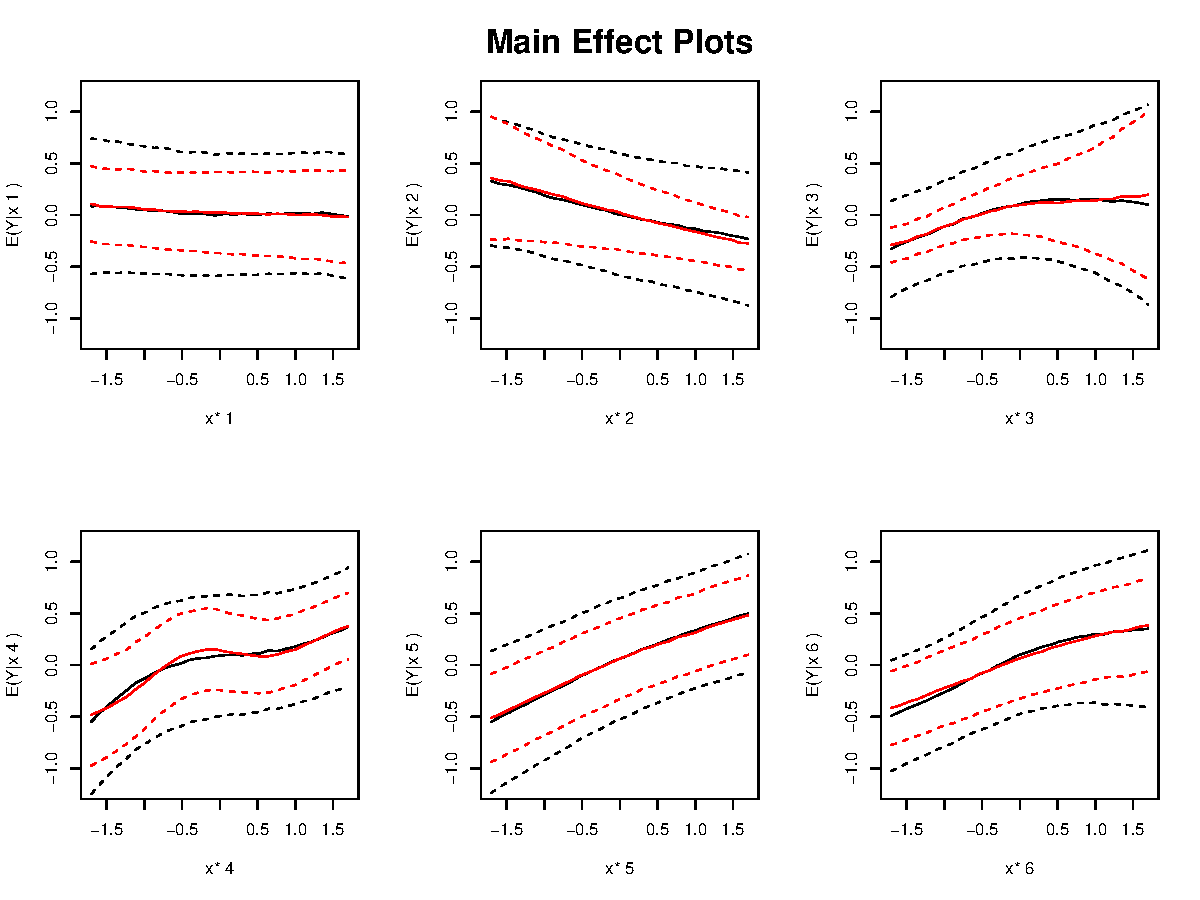
\includegraphics[width = 0.9\textwidth]{fig-sa/main-effects.pdf}
	\caption{Main effect curves (solid) $\pm 2$ standard deviations (dashed). Black represents HetGP and red is SML emulation.}
	\label{Fig:main-effect}
\end{figure}

In \Cref{Fig:main-effect} we see that the effect curves are similar for both HetGP and SML. However, the uncertainty bands are quite different. In this case, the uncertainty bands are calculated in a similar way to the main effects, we integrate the variance over $G_{-i|i}(X_{-i}|X_i)$. Further, these uncertainty bands represent out ``total'' uncertainty in prediction - they are a combination of the uncertainty in the mean function but also the stochastic nature of the simulator, so give us (approximate) $95\%$ probability bands for a new simulator run, if we were to learn the value of $x_i$. We see that variables $4$ --- $6$ are the most influential, which suggests that the best way to have a windfarm with high availability is to have well functioning components.

\section{Choice of Prior}

To perform the sensitivity analysis, we must specify a distribution, $G$. As mentioned by \citet{Marrel2012}, the model inputs must be deemed as independent in this screening process to ensure a unique ANOVA decomposition of the simulator. We will now perform an investigation into the choice of $G$ subject to a few constraints:\\

\begin{itemize}
	\item Each choice of $G$ has the same mean.
	\item Each choice of $G$ is symmetric.
	\item Each choice of $G$ has a similar $0.05\%$ and $99.5\%$ quantiles.
\end{itemize}

The analysis above used uniform priors over the range of the observed data. However, using a distribution with a hard cut-off may not be satisfactory. For instance, the uncertain input in question could plausibly take any value on the real line, but we just believe that it is likely to be between two limits. We will experiment with a choice of two symmetric, unimodal choice of $G$. First we will try $G(x^*_i) \sim \mathcal{N}(0,0.65^2)$. We will also try $G(X^*_i) \sim 0.536t_{10} $. These were chosen since they give $P(-1.7 < x^*_i < 1.7) = 0.99$. The uniform priors from before have the property $P(-1.7 < x^*_i <1.7) = 1$, so these distributions have similar quantiles. They are also all symmetric, unimodal and have mean $0$. Therefore, each of these priors have many similar summaries. They could all be deemed as an adequate (coarse) representation of beliefs by an expert.\\

We then compute the first order sensitivity indices and $S_{T_\varepsilon}$ via a simple MC method. We can then compare the values of the indices to gauge the relative importance of each variable under different prior specifications.

\begin{table}[ht]
\centering
\begin{tabular}{rrrrrrrr}
  \toprule
 $G$ & $100\hat{S}_1$ & $100\hat{S}_2$ & $100\hat{S}_3$ & $100\hat{S}_4$ & $100\hat{S}_5$ & $100\hat{S}_6$ & $100\hat{S}_{T_\varepsilon}$\\ 
  \cmidrule{1-8}
$\mathcal{U}$ & $0.72$ & $8.18$ & $5.96$ & $13.88$ & $29.17$ & $22.20$ & $13.81$\\ 
  $\mathcal{N}$ & $0.36$ & $7.87$ & $8.56$ & $7.24$ & $25.96$ & $27.12$ & $15.85$\\ 
  $t_{10}$ & $0.50$ & $7.82$ & $9.12$ & $6.28$ & $25.25$ & $28.41$ & $16.96$\\ 
   \bottomrule
\end{tabular}
\caption{Estimated first order sensitivity indices and $S_{T_\varepsilon}$ for three simple choices of $G$.}
\label{Tab:sa-sensitivity}
\end{table}
%% references 


From \Cref{Tab:sa-sensitivity} we see that for the $t_{10}$ and Normal priors, $S_6 >  S_5 > S_3 > S_2 > S_4 > S_1$ whereas for the uniform prior $S_5 > S_6 > S_4 > S_2 > S_3 > S_1$. The only real agreement between these two formulations is that they both rank $S_1$ as the least informative first order effect. They all rank $S_5$ and $S_6$ as the two most important first order effects. The row sums for the above table are $93.92,$ $92.96$ and $94.34$ respectively (top --- bottom). Therefore, in each case the interactions between controllable variables have a similar effect; of the order of $5\% - 7\%$.

\section{Using Sensitivity Indices to Guide Probability Elicitation}

A sensitivity is very useful to guide a facilitator in probability elicitation. The SHELF procedure \citep{SHELF4} suggests that the most time and effort should be spent on the elicitation of the most important parameters. What is ``important'' will depend on the context. Many would agree that if an input variable in a computer model contributes to a lot of the variation in the output then it would be deemed important. The sensitivity indices allow us to quantify ``importance'' in an intuitive manner. The sensitivity indices are not the only consideration, but they are  a useful tool nonetheless.\\

\Cref{Fig:elicitation-flowchart} provides an illustration of how an emulator-assisted sensitivity analysis can be used to guide an elicitation involving a complex computer model.
\begin{figure}

\begin{center}
\resizebox{0.4\textwidth}{!}{
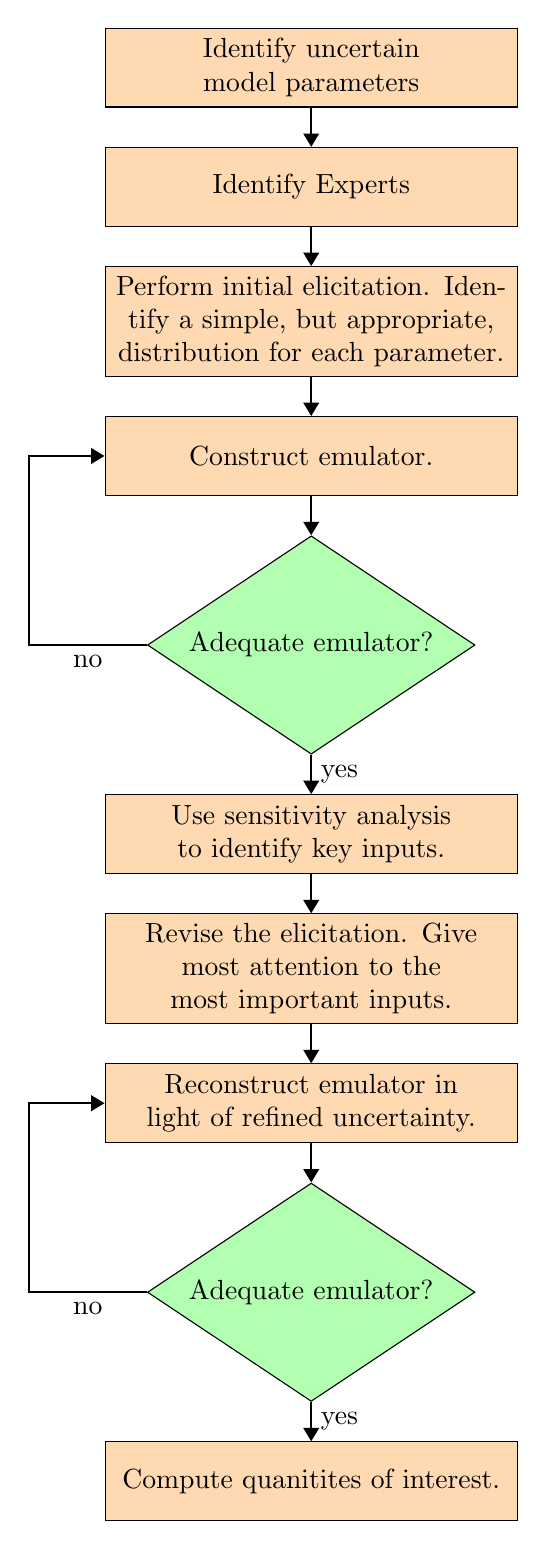
\begin{tikzpicture}[FlowChart,                   % used are styles from tikzset FlowChart
    node distance = 5mm and 7mm,
      start chain = A going below                    % The nodes in the chain
                                                     % will be named by A-1, A-2, ...
                        ]
\node   [process] {Identify uncertain model parameters};               % A-1
\node   [process]   {Identify Experts}; %A-2
\node   [process]   {Perform initial elicitation. Identify a simple, but appropriate, distribution for each parameter.};%A-3
\node   [process]   {Construct emulator.};%A-4
\node   [decision] {Adequate emulator?};%A-5
\node   [process]   {Use sensitivity analysis to identify key inputs.};%A-6
\node   [process]   {Revise the elicitation. Give most attention to the most important inputs.};%A-7
\node   [process]   {Reconstruct emulator in light of refined uncertainty.};%A-8
\node   [decision] {Adequate emulator?};%A-9
\node   [process]   {Compute quanitites of interest.};%A-10
% lines not considered by join macro
\draw [arrow] (A-5.west) to ["no"] ++ (-1.5,0) |- (A-4);
\path   (A-5) to ["yes"] (A-6);
\draw [arrow] (A-9.west) to ["no"] ++ (-1.5,0) |- (A-8);
\path   (A-9) to ["yes"] (A-10);
    \end{tikzpicture}
}
\end{center}

\caption{Illustration of how emulators and sensitivity analysis can be used to assist the elicitation for forward uncertainty propagation.}
\label{Fig:elicitation-flowchart}
\end{figure}
\end{chapter}
